\chapter{Intonation questionnaires}\label{app:a}
\section{Italian version}\label{app:a1}

\begin{xltabular}{\textwidth}{lQQ}
\lsptoprule Nr. & Context\slash Given answer & Translation\\\midrule\endfirsthead
\midrule Nr. & Context\slash Given answer & Translation\\\midrule\endhead
\endfoot\lspbottomrule\endlastfoot

01 & Ti chiedono che frutta preferisci. Tu rispondi che preferisci i mandarini. (Che frutta preferisci?)

-- \textit{Preferisco i mandarini.} & They ask you what fruit you prefer. You say that you prefer tangerines. (What fruit do you prefer?)

{\itshape -- I prefer tangerines.}\\
\tablevspace
02 & Guardati la foto e dimmi: che cosa sta succedendo?

-- \textit{Marisa mangia dei mandarini.} & Look at the picture and tell me what is happening here.

-- \textit{Marisa is eating tangerines.}

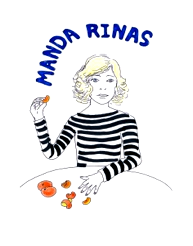
\includegraphics[width=.3\textwidth]{figures/a08HabilAppendix-img001.png}
 (Marisa)\\
\tablevspace
03 & Dimmi i giorni della settimana.

-- \textit{Lunedì, Martedì, Mercoledì, Giovedì, Venerdì, Sabato e Domenica.} & Tell me the days of the week.

{\itshape -- Monday, Tuesday, Wednesday, Thursday, Friday, Saturday, Sunday.}\\
%\tablevspace
04 & Entri in un commercio, dove lavora una commessa un po' sorda. Le dici che vuoi alcune arance. Lei ti chiede se desideri limoni... (Desidera limoni?)

{\itshape -- No, arance!} & You enter a store where the saleswoman is a little hard of hearing. You tell her that you would like a kilo of oranges, but she doesn’t hear you well and asks you if you want lemons. Tell her that you want oranges.

{\itshape -- No, oranges!}\\
\tablevspace
05 & Sei con un amico e gli dici che la vostra amica Maria fa un viaggio di nozze. Lui ti chiede con chi. Ti sorprende molto che non lo sappia, perché tutti sanno che con il suo fidanzato, ormai marito, sia Manuele.

\textit{-- Con Manuele!} & You are with a friend and you explain to him/her that Mary, a mutual friend of yours, is getting married. Your friend asks you who she is marrying. You're surprised that s/he doesn’t know, because everyone knows that Mary is planning to marry her long-time boyfriend, Manuel. Tell him/her that she’s getting married to Manuel.

{\itshape -- To Manuel (obviously)!}\\
\tablevspace
06 & I tuoi bambini vanno a dormire. Che cosa gli dici?

-- \textit{Buona notte, bambini!} & Your children are in bed, ready to go to sleep. What do you say to them?

{\itshape -- Good night, kids!}\\
\tablevspace
07 & Entri in un negozio dove non sei mai stato prima e chiedi se hanno dei mandarini.

{\itshape -- Avete dei mandarini?} & You enter a store that you have never been in before and ask if they have any tangerines.

-- \textit{Have you got tangerines?}\\
\tablevspace
08 & Proprio adesso hai pranzato molto con un amico e vedi che lui si ferma davanti alla pasticceria. Chiedi (molto sorpreso, perché avete finito il pranzo) se ancora ha fame.

{\itshape -- Hai ancora fame?} & You have just finished lunch with a friend and you see that he seems to have stopped in front of a pastry shop. Amazed -- since he just ate a big meal -- you ask him if he is still hungry.

-- \textit{You’re still hungry?}\\
%\tablevspace
09 & I tuoi nipoti fanno un sacco di rumore e non ti lasciano guardare la TV. Gli chiedi se possono rimanere zitti.

\textit{-- Volete rimanere zitti?} & Your nieces and nephews are making lots of noise and you can’t hear the television.~You ask them to be quiet.

-- \textit{Will you be quiet?}\\
\tablevspace
10 & Chiedi al tuo amico se vuole andare a prendere una birra con te.

{\itshape -- Andiamo a prendere una birra?} & Propose to a friend that the two of you go out for a beer.

-- \textit{Shall we go for a beer?}\\
\tablevspace
11 & Sali sul bus. C'è un posto libero accanto a una signora. Chiedi se puoi sederti.

-- \textit{Scusi, posso sedermi?} & You are on the bus and want to sit down next to an older woman. You ask her politely if the seat next to her is available and if you may sit down.

{\itshape -- Excuse me, may I sit down?}\\
\tablevspace
12 & Conosci una ragazza. Chiedi come si chiama.

{\itshape -- Come ti chiami?} & You meet somebody for the first time. Ask her/him what her/his name is.

{\itshape -- What is your name?}\\
\tablevspace
13 & Sei in una grande città per la prima volta. Vuoi andare alla chiesa di Sant’Antonio. Chiedi ad un signore per strada dove si trova.

{\itshape -- Dove si trova la chiesa di Sant’Antonio?} & You are in a big city for the first time. You want to go to the San Antonio Church. Ask a man on the street where it is.

{\itshape -- Where is the San Antonio Church?}\\
\tablevspace
14 & Hai un appuntamento con il tuo amico ma avevi dimenticato l'orologio a casa. Chiedi ad una signora che ora è….

\textit{-- Che ora è?} & You have an appointment with a friend of yours but forgot your watch and mobile at home. Ask an older woman on the street what time it is.

{\itshape -- What time is it?}\\
%\tablevspace
15 & Fai vedere a un amico una foto di un attore molto famoso. Il tuo amico ti chiede chi è. Ti sorprende la sua domanda, perché tutti lo conoscono.

{\itshape -- Ma come? È John Travolta!} & You show a picture of a very famous actor to your friend. (S)he asks you who it is. This surprises you, because everybody knows him. How do you react?

{\itshape -- It is John Travolta (obviously)!}\\
\tablevspace
16 & Sei invitato a cenare a casa di un amico. Quando arrivi, senti un buon odore di cucina. Che cosa dici al tuo amico?

{\itshape -- Oh, che buon profumino!} & You are invited for a dinner at your friend’s place and when you arrive you smell a delicious aroma. What do you say to your friend?

{\itshape -- Mmm! How good it smells!}\\
\tablevspace
17 & Tua figlia di quindici anni torna a casa alle due di notte. Sei molto arrabbiata perché non sai dove è stata, con chi etc. Che cosa le domandi?

{\itshape -- Dove sei stata?} & Your fifteen-year-old daughter returns home at 2 o’clock in the morning. You are very upset because you did not know where she was, with whom, etc. How do you react?

{\itshape -- Where have you been?}\\
\tablevspace
18 & Qualcuno bussa alla porta. Apri, è il tuo amico Roberto che non vedi da molti anni. Come reagisci?

{\itshape -- Ciao, Roberto! Che sorpresa!} & Somebody knocks on the door. You open it and there is your friend Robert. You have not seen him for years. How do you react?

{\itshape -- Hello, Robert. What a surprise!}\\
\tablevspace
19 & C'è un tipo strano nel tuo quartiere che ti dà sempre fastidio e quando ti trova non ti lascia in pace. Oggi è la terza volta che ti chiama per telefono. Chiedigli che cosa vuole...

{\itshape -- Cosa vuole?} & There is a strange man in your neighbourhood who always annoys you, and whenever he runs into you, he won’t leave you alone. Today it is already the third time that he has run into you. Ask him what he wants.

{\itshape -- What do you want?}\\
%\tablevspace
20 & La tua vicina ti dice che è andata a mangiare in un ristorante e ha ordinato il coniglio con le cipolle. Convinta, ti dice che le hanno servito un gatto al posto del coniglio. Non le puoi credere. Chiedi che cosa le hanno servito (molto molto sorpresa.)

\textit{-- Cosa ti hanno servito?} & Your neighbour tells you that she had dinner at a restaurant and ordered rabbit with onion. However, she is utterly convinced that they gave her cat meat instead of rabbit. You find this extremely difficult to believe, so you ask her to confirm what they gave her.

{\itshape -- They served you what?}\\
\tablevspace
21 & Ti dicono che il tuo amico Giovanni si è presentato per la carica di presidente. Non ci puoi credere e chiedi di nuovo.

\textit{-- Giovanni? Presidente?} & You hear that, John, a friend of yours, is running for president. You can’t believe it and ask again.

{\itshape -- John? For president?}\\
\tablevspace
22 & Sei nel parco con tua nipote Natalia. Improvvisamente, lei inizia a correre e vuole uscire dal parco. Ti spaventi perché accanto al parco c'è una strada dove passano molte macchine. Dille di venire da te.

{\itshape -- Naty, vieni qui!} & You are at the park with your little niece Natalia. She is running and gets further and further from you.~You are alarmed because there is heavy traffic on the avenue that runs alongside the park. You tell her to come back.

{\itshape -- Naty, come here!}\\
\tablevspace
23 & Sei una receptionist in un albergo. È venuta una coppia e vuole un’abitazione. Digli di compilare il modulo.

{\itshape -- Compilate il modulo, per favore.} & Imagine that you are a receptionist at a hotel, and a couple enters and wants a room. Tell them to fill out a form.

{\itshape -- Please fill out the form.}\\
%\tablevspace
24 & Vuoi andare al cinema con un amico. Lui ti dice che deve lavorare, ma tu sai che può saltare per un altro giorno. Come fai a convincerlo? Digli di venire.

{\itshape -- Dai, per favore, vieni al cinema con me!} & You want to go to the movies with a friend. Your friend tells you that s/he has work that s/he needs to do, but you know that s/he can leave it for later. What do you say to convince him/her to accompany you?

{\itshape -- Come on!, Come to the cinema with me!}\\
\tablevspace
25 & Passi per la città e vedi la tua amica Natalia sull'altro lato della strada. Chiamala.

\textit{-- Natalia!} & You see Natalia, a friend of yours, on the other side of the street. Call her.

\textit{-- Natalia!}\\
\end{xltabular}




\section{Spanish version}\label{app:a2}




\begin{xltabular}{\textwidth}{lQQ}
\lsptoprule
Nr. & Context\slash Given answer & Translation\\\midrule\endfirsthead
\midrule Nr. & Context\slash Given answer & Translation\\\midrule\endhead
\endfoot\lspbottomrule\endlastfoot
01 & Te preguntan qué fruta prefieres. Dices que prefieres mandarinas. (¿Qué fruta prefieres?)

-- \textit{Prefiero mandarinas.} & They ask you what fruit you prefer. You say that you prefer tangerines. (What fruit do you prefer?)

{\itshape -- I prefer tangerines.}\\
%\tablevspace
02 & Mira el dibujo y dime: ¿qué pasa aquí?

-- \textit{Marisa come mandarinas.} & Look at the picture and tell me what is happening here.

-- \textit{Marisa is eating tangerines.}


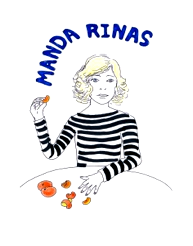
\includegraphics[width=.3\textwidth]{figures/a08HabilAppendix-img001.png}
 (Marisa)\\
 \tablevspace
03 & Dime los días de la semana.

-- \textit{Lunes, martes, miércoles, jueves, viernes, sábado y domingo.} & Tell me the days of the week.

{\itshape -- Monday, Tuesday, Wednesday, Thursday, Friday, Saturday, Sunday.}\\
\tablevspace
04 & Entras en una frutería donde hay una vendedora un poco sorda. Le dices que quieres un par de naranjas. Ella te pregunta si son limones, lo que quieres.

\textit{-- ¡No, naranjas!} & You enter a store where the saleswoman is a little hard of hearing. You tell her that you would like a kilo of oranges, but she doesn’t hear you well and asks you if you want lemons. Tell her that you want oranges.

{\itshape -- No, oranges!}\\
%\tablevspace
05 & Estás con una amiga y le dices que vuestra amiga María se va a casar. Ella te pregunta con quién. A ti te sorprende mucho que no lo sepa, porque todo el mundo sabe que con su novio, Manuel.

\textit{-- ¡Con Manuel!} & You are with a friend and you explain to him/her that Mary, a mutual friend of yours, is getting married. Your friend asks you who she is marrying. You're surprised that s/he doesn’t know, because everyone knows that Mary is planning to marry her long-time boyfriend, Manuel. Tell him/her that she’s getting married to Manuel.

{\itshape -- To Manuel (obviously)!}\\
\tablevspace
06 & Tus hijos se van a dormir. ¿Qué les dices?

-- \textit{¡Buenas noches, niños!} & Your children are in bed, ready to go to sleep. What do you say to them?

\textit{-- Good night, kids!}\\
\tablevspace
07 & Entras en una tienda y preguntas si tienen mandarinas.

\textit{-- ¿Tienen mandarinas?} & You enter a store that you have never been in before and ask if they have any tangerines.

-- \textit{Have you got tangerines?}\\
\tablevspace
08 & Acabas de cenar con un amigo y ves que él se para delante de la pastelería. Pregúntale (todo asombrado porque acabaron de cenar) si todavía tiene hambre.

\textit{-- ¿Todavía tienes hambre?} & You have just finished lunch with a friend and you see that he seems to have stopped in front of a pastry shop. Amazed -- since he just ate a big meal -- you ask him if he is still hungry.

-- \textit{You’re still hungry?}\\
\tablevspace
09 & Tus sobrinos hacen mucho ruido y no te dejan escuchar la televisión. Les preguntas si se quieren callar.

\textit{-- ¿Quieren callarse?} & Your nieces and nephews are making lots of noise and you can’t hear the television.~You ask them to be quiet.

-- \textit{Will you be quiet?}\\
\\
10 & Pregúntale a tu amigo si quiere ir a tomar una cerveza contigo.

\textit{-- ¿Vamos a tomar una cerveza?} & Propose to a friend that the two of you go out for a beer.

-- \textit{Shall we go for a beer?}\\
\tablevspace
11 & Estás en el autobús. Hay un asiento libre al lado de una señora mayor. Le preguntas si puedes sentarte.

-- \textit{Permiso, ¿me puedo sentar?} & You are on the bus and want to sit down next to an older woman. You ask her politely if the seat next to her is available and if you may sit down.

{\itshape -- Excuse me, may I sit down?}\\
\tablevspace
12 & Acabas de conocer a una chica. Pregúntale cómo se llama.

\textit{-- ¿Cómo te llamas?} & You meet somebody for the first time. Ask her/him what her/his name is.

{\itshape -- What is your name?}\\
\tablevspace
13 & Estás en una ciudad grande por primera vez. Quieres ir a la iglesia de San Antonio. Pregúntale a un señor en la calle dónde está.

\textit{-- ¿Dónde está la iglesia de San Antonio?} & You are in a big city for the first time. You want to go to the San Antonio Church. Ask a man on the street where it is.

{\itshape -- Where is the San Antonio Church?}\\
\tablevspace
14 & Tienes una cita con tu amigo y has dejado tu reloj en casa. Pregúntale a una señora qué hora es.

\textit{-- ¿Qué hora es?} & You have an appointment with a friend of yours but forgot your watch and mobile at home. Ask an older woman on the street what time it is.

{\itshape -- What time is it?}\\
\tablevspace
15 & Le enseñas a un amigo tuyo una foto con un actor muy famoso. Tu amigo te pregunta quién es. A ti te sorprende la pregunta porque todo el mundo lo conoce.

\textit{-- ¡Es John Travolta!} & You show a picture of a very famous actor to your friend. (S)he asks you who it is. This surprises you, because everybody knows him. How do you react?

{\itshape -- It is John Travolta (obviously)!}\\
\\
16 & Estás invitado a cenar a casa de un amigo. Cuando llegues, sientes un buen olor de cocina. ¿Cómo se lo dices a tu amigo?

\textit{-- ¡Ay, qué rico olor!} & You are invited for a dinner at your friend’s place and when you arrive you smell a delicious aroma. What do you say to your friend?

{\itshape -- Mmm! How good it smells!}\\
\tablevspace
17 & Tu hija de quince años regresa a casa a las dos de la noche. Estás muy enfadada porque no sabías dónde estaba, con quién etc. ¿Qué le preguntas?

\textit{-- ¿Dónde estuviste?} & Your fifteen-year-old daughter returns home at 2 o’clock in the morning. You are very upset because you did not know where she was, with whom, etc. How do you react?

{\itshape -- Where have you been?}\\
\tablevspace
18 & Alguien toca a la puerta. Abres y es tu amigo Roberto. Hace años que no lo ves. ¿Cómo reaccionas?

\textit{-- ¡Hola, Roberto! ¡Qué sorpresa!} & Somebody knocks on the door. You open it and there is your friend Robert. You have not seen him for years. How do you react?

{\itshape -- Hello, Robert. What a surprise!}\\
\tablevspace
19 & Hay un tipo raro en tu barrio que siempre te molesta y cuando te encuentra nunca te deja en paz. Hoy ya es la tercera vez que te llama por teléfono. Pregúntale qué quiere...

\textit{-- ¿Qué quieres?} & There is a strange man in your neighbourhood who always annoys you, and whenever he runs into you, he won’t leave you alone. Today it is already the third time that he has run into you. Ask him what he wants.

{\itshape -- What do you want?}\\
\tablevspace
20 & Tu vecina te cuenta que fue a comer a un restaurante y pidió conejo con cebolla. Muy convencida te dice que le sirvieron un gato en vez del conejo. No lo puedes creer. Pregúntale qué le sirvieron (muy muy sorprendida.)

\textit{-- ¿Qué te sirvieron?} & Your neighbour tells you that she had dinner at a restaurant and ordered rabbit with onion. However, she is utterly convinced that they gave her cat meat instead of rabbit. You find this extremely difficult to believe, so you ask her to confirm what they gave her.

{\itshape -- They served you what?}\\
%\tablevspace
21 & Te dicen que un amigo tuyo, Juan, se presenta para el puesto de presidente. No lo puedes creer y vuelves a preguntar.

\textit{-- ¿Juan? ¿Presidente?} & You hear that, John, a friend of yours, is running for president. You can’t believe it and ask again.

{\itshape -- John? For president?}\\
\tablevspace
22 & Estás en el parque con tu sobrina Natalia. De repente, ella echa a correr y sale del parque. Te asustas porque al lado del parque hay una avenida por donde pasan muchos coches. Dile que venga.

\textit{-- ¡Naty, ven aquí!} & You are at the park with your little niece Natalia. She is running and gets further and further from you.~You are alarmed because there is heavy traffic on the avenue that runs alongside the park. You tell her to come back.

{\itshape -- Naty, come here!}\\
\tablevspace
23 & Eres recepcionista en un hotel. Ha llegado una pareja y quieren una habitación. Diles que completen el formulario.

\textit{-- Completen el formulario, por favor.} & Imagine that you are a receptionist at a hotel, and a couple enters and wants a room. Tell them to fill out a form.

{\itshape -- Please fill out the form.}\\
\tablevspace
24 & Quieres ir al cine con un amigo. Te dice que tiene que trabajar, pero sabes que lo puede dejar para otro día. ¿Cómo lo convences? Dile que venga.

\textit{-- ¡Por favor, ven conmigo al cine!} & You want to go to the movies with a friend. Your friend tells you that s/he has work that s/he needs to do, but you know that s/he can leave it for later. What do you say to convince him/her to accompany you?

{\itshape -- Come on!, Come to the cinema with me!}\\
\tablevspace
25 & Pasas por la ciudad y ves a tu amiga Natalia en el otro lado de la calle. Llámala.

\textit{-- ¡Natalia!} & You see Natalia, a friend of yours, on the other side of the street. Call her.

\textit{-- Natalia!}\\
\end{xltabular}

\newpage
\section{Czech version}\label{app:a3}
\begin{xltabular}{\textwidth}{lQQ}
\lsptoprule Nr. & Context\slash Given answer & Translation\\\midrule\endfirsthead
\midrule Nr. & Context\slash Given answer & Translation\\\midrule\endhead
\endfoot\lspbottomrule\endlastfoot
01 & Zeptají se Tě, jaké máš rád ovoce. Odpovíš, že mandarinky. (Jaké máš rád ovoce?)

-- \textit{Já mám rád mandarinky.} & They ask you what fruit you prefer. You say that you prefer tangerines. (What fruit do you prefer?)

{\itshape -- I prefer tangerines.}\\
\tablevspace
02 & Podívej se na obrázek a řekni mi, co se na něm děje.

-- \textit{Marisa jí mandarinky.} & Look at the picture and tell me what is happening here.

-- \textit{Marisa is eating tangerines.}


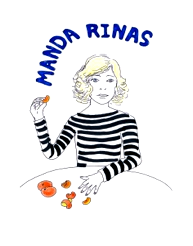
\includegraphics[width=.3\textwidth]{figures/a08HabilAppendix-img001.png}
 (Marisa)\\
 \tablevspace
03 & Vyjmenuj dny v týdnu.

-- \textit{Pondělí, úterý, středa, čtvrtek, pátek, sobota a neděle.} & Tell me the days of the week.

{\itshape -- Monday, Tuesday, Wednesday, Thursday, Friday, Saturday, Sunday.}\\
\tablevspace
04 & Vejdeš do obchůdku s ovocem a zeleninou, ve kterém prodává starší nahluchlá paní. Chceš koupit pomeranče, ale paní se Tě zeptá, jestli chceš citrony, protože neslyšela dobře. (Přejete si citrony?)

{\itshape -- Ne, pomeranče!} & You enter a store where the saleswoman is a little hard of hearing. You tell her that you would like a kilo of oranges, but she doesn’t hear you well and asks you if you want lemons. Tell her that you want oranges.

{\itshape -- No, oranges!}\\
%\tablevspace
05 & Mluvíš s kamarádem o Marii, vaší dobré kamarádce. Řekneš, že se bude vdávat. On se tě zeptá, koho si bude brát. Tebe to překvapí, protože všichni ví, že si bere Manuela, svého dlouhodobého přítele. (A koho si bere?).

{\itshape -- No přece Manuela!} & You are with a friend and you explain to him/her that Mary, a mutual friend of yours, is getting married. Your friend asks you who she is marrying. You're surprised that s/he doesn’t know, because everyone knows that Mary is planning to marry her long-time boyfriend, Manuel. Tell him/her that she’s getting married to Manuel.

{\itshape -- To Manuel (obviously)!}\\
\tablevspace
06 & Tvé děti jdou spát. Co jim řekneš?

-- \textit{Dobrou noc, děti!} & Your children are in bed, ready to go to sleep. What do you say to them?

{\itshape -- Good night, kids!}\\
\tablevspace
07 & Vejdeš do jednoho obchodu úplně poprvé a zeptáš se, jestli mají mandarinky.

{\itshape -- Máte mandarinky?} & You enter a store that you have never been in before and ask if they have any tangerines.

-- \textit{Have you got tangerines?}\\
\tablevspace
08 & Vracíš se s kamarádem z vydatného oběda a vidíš, že se zastavil před cukrárnou. Zeptej se ho (udiveně, protože jste právě hodně pojedli), zda má ještě hlad.

{\itshape -- Ty máš ještě hlad?} & You have just finished lunch with a friend and you see that he seems to have stopped in front of a pastry shop. Amazed -- since he just ate a big meal -- you ask him if he is still hungry.

-- \textit{You’re still hungry?}\\
\tablevspace
09 & Děti dělají strašný rámus a nenechají tě dívat se na televizi. Zeptej se jich, jestli budou zticha.

\textit{-- Budete už zticha?} & Your nieces and nephews are making lots of noise and you can’t hear the television.~You ask them to be quiet.

-- \textit{Will you be quiet?}\\
\\
10 & Zeptej se kamaráda, jestli půjde s tebou na pivo.

\textit{-- Jdeme na pivo?} & Propose to a friend that the two of you go out for a beer.

-- \textit{Shall we go for a beer?}\\
\tablevspace
11 & Jsi v autobuse a vedle jedné paní je jedno volné místo. Zeptej se jí, jestli má vedle sebe volno.

-- \textit{Promiňte, prosím, je tady volno?} & You are on the bus and want to sit down next to an older woman. You ask her politely if the seat next to her is available and if you may sit down.

{\itshape -- Excuse me, may I sit down?}\\
\tablevspace
12 & Právě se s někým seznámíš. Zeptej se, jak se jmenuje.

{\itshape -- Jak se jmenuješ?} & You meet somebody for the first time. Ask her/him what her/his name is.

{\itshape -- What is your name?}\\
\tablevspace
13 & Jsi poprvé v jednom městě a hledáš kostel Svatého Antonína. Zeptej se, kde je.

{\itshape -- Kde je tady kostel Svatého Antonína?} & You are in a big city for the first time. You want to go to the San Antonio Church. Ask a man on the street where it is.

{\itshape -- Where is the San Antonio Church?}\\
\tablevspace
14 & Máš s kamarádem schůzku, ale zapomněl(a) sis doma hodinky. Zeptej se někoho, kolik je hodin.

{\itshape -- Kolik je hodin?} & You have an appointment with a friend of yours but forgot your watch and mobile at home. Ask an older woman on the street what time it is.

{\itshape -- What time is it?}\\
\tablevspace
15 & Kamarádovi ukážeš fotku s jedním velmi známým hercem. On se tě zeptá, kdo to je. Tebe to překvapí, protože ho každý zná.

{\itshape -- To je John Travolta!} & You show a picture of a very famous actor to your friend. (S)he asks you who it is. This surprises you, because everybody knows him. How do you react?

{\itshape -- It is John Travolta (obviously)!}\\
%\tablevspace
16 & Kamarád tě pozve domů na večeři. Když přijdeš, bytem se line hezká vůně. Jak zareaguješ?

{\itshape -- To ale hezky voní!} & You are invited for a dinner at your friend’s place and when you arrive you smell a delicious aroma. What do you say to your friend?

{\itshape -- Mmm! How good it smells!}\\
\tablevspace
17 & Tvoje patnáctiletá dcera se vrátí ve tři hodiny ráno. Jsi dost naštvaný, protože jsi nevěděl, kde byla, a dělal sis velké starosti. Co jí řekneš?

\textit{-- Kde jsi byla?} & Your fifteen-year-old daughter returns home at 2 o’clock in the morning. You are very upset because you did not know where she was, with whom, etc. How do you react?

{\itshape -- Where have you been?}\\
\tablevspace
18 & Někdo zvoní. Otevřeš a ve dveřích stojí kamarád Robert, kterého jsi dlouho neviděl(a). Jak zareaguješ?

{\itshape -- Ahoj, Roberte! To je ale překvapení!!} & Somebody knocks on the door. You open it and there is your friend Robert. You have not seen him for years. How do you react?

{\itshape -- Hello, Robert. What a surprise!}\\
\tablevspace
19 & V tvém domě bydlí jeden podivný starší pán, který tě nikdy nenechá na pokoji. Dnes už je to počtvrté, co ti volá a otravuje. Zeptej se ho, co chce...

\textit{-- Co chcete?} & There is a strange man in your neighbourhood who always annoys you, and whenever he runs into you, he won’t leave you alone. Today it is already the third time that he has run into you. Ask him what he wants.

{\itshape -- What do you want?}\\
\tablevspace
20 & Tvoje sousedka ti vypraví, že byla na večeři a objednala si králíka na cibulce. Úplně přesvědčivě ti řekne, že ji přinesli kočku. Tebe to zaskočí a zeptáš se ještě jednou, cože jí to přinesli (dost udiveně).)

\textit{-- Cože ti to přinesli?} & Your neighbour tells you that she had dinner at a restaurant and ordered rabbit with onion. However, she is utterly convinced that they gave her cat meat instead of rabbit. You find this extremely difficult to believe, so you ask her to confirm what they gave her.

{\itshape -- They served you what?}\\
%\tablevspace
21 & Kamarád ti vypraví, že Jan, váš kamarád, kandiduje na prezidenta. Tebe to šokuje. Co řekneš?

\textit{-- Jan? Na prezidenta?} & You hear that, John, a friend of yours, is running for president. You can’t believe it and ask again.

{\itshape -- John? For president?}\\
\tablevspace
22 & Jsi v parku s Natálkou. Ona se najednou rozběhne k východu. Ty se lekneš, protože vedle parku je velmi rušná silnice. Řekni, ať přijde.

{\itshape -- Naty, pojď sem!} & You are at the park with your little niece Natalia. She is running and gets further and further from you.~You are alarmed because there is heavy traffic on the avenue that runs alongside the park. You tell her to come back.

{\itshape -- Naty, come here!}\\
\tablevspace
23 & Pracuješ v hotelové recepci. Přijde jeden pár a žádá si pokoj. Řekni, ať vyplní daný formulář.

{\itshape -- Vyplňte, prosím, tento formulář.} & Imagine that you are a receptionist at a hotel, and a couple enters and wants a room. Tell them to fill out a form.

{\itshape -- Please fill out the form.}\\
\tablevspace
24 & Chceš jít s kamarádem do kina. Řekne ti, že musí pracovat, ty ale víš, že to může nechat na jindy. Jak ho přesvědčíš? Popros, ať jde s tebou.

{\itshape -- No tak, pojď se mnou do kina!} & You want to go to the movies with a friend. Your friend tells you that s/he has work that s/he needs to do, but you know that s/he can leave it for later. What do you say to convince him/her to accompany you?

{\itshape -- Come on!, Come to the cinema with me!}\\
\tablevspace
25 & Jdeš po městě a na druhé straně ulice vidíš svoji kamarádku Natálii. Zavolej ji.

\textit{-- Natálie!} & You see Natalia, a friend of yours, on the other side of the street. Call her.

\textit{-- Natalia!}\\
\end{xltabular}

\newpage
\section{German version}\label{app:a4}


\begin{xltabular}{\textwidth}{lQQ}

\lsptoprule
Nr. & Context\slash Given answer & Translation\\
\midrule
\endfirsthead
    \midrule
Nr. & Context\slash Given answer & Translation\\
		\midrule\endhead
    \endfoot
    \lspbottomrule
    \endlastfoot
01 & Du wirst gefragt, welches deine Lieblingsfrüchte sind. Du sagst, dass du Mandarinen magst.

-- \textit{Ich mag Mandarinen.} & They ask you what fruit you prefer. You say that you prefer tangerines. (What fruit do you prefer?)

{\itshape -- I prefer tangerines.}\\
\tablevspace
02 & Sieh dir das Bild an und beschreibe, was passiert.

-- \textit{Marisa isst Mandarinen.} & Look at the picture and tell me what is happening here.

-- \textit{Marisa is eating tangerines.}

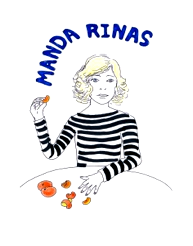
\includegraphics[width=.3\textwidth]{figures/a08HabilAppendix-img001.png}
 (Marisa)\\
\tablevspace
03 & Sag die Wochentage auf.

-- \textit{Montag, Dienstag, Mittwoch, Donnerstag, Freitag, Samstag und Sonntag.} & Tell me the days of the week.

{\itshape -- Monday, Tuesday, Wednesday, Thursday, Friday, Saturday, Sunday.}\\
\tablevspace
04 & Du gehst in einen Obst- und Gemüseladen und die Verkäuferin ist ein bisschen schwerhörig. Du sagst ihr, dass du ein paar Orangen möchtest. Sie fragt dich, ob es Zitronen sind, die du möchtest.

-- \textit{Nein, Orangen!} & You enter a store where the saleswoman is a little hard of hearing. You tell her that you would like a kilo of oranges, but she doesn’t hear you well and asks you if you want lemons. Tell her that you want oranges.

{\itshape -- No, oranges!}\\
%\tablevspace
05 & Du unterhälst dich mit einer Freundin und erzählst ihr, dass eure gemeinsame Freundin Maria heiraten wird. Sie fragt dich wen sie heiratet. Du bist sehr überrascht, dass sie es nicht weiß, da jeder weiß, dass sie ihren Freund, Manuel, heiratet.

\textit{-- Manuel!} & You are with a friend and you explain to him/her that Mary, a mutual friend of yours, is getting married. Your friend asks you who she is marrying. You're surprised that s/he doesn’t know, because everyone knows that Mary is planning to marry her long-time boyfriend, Manuel. Tell him/her that she’s getting married to Manuel.

{\itshape -- To Manuel (obviously)!}\\
\tablevspace
06 & Deine Kinder gehen ins Bett. Was sagst du zu ihnen?

-- \textit{Gute Nacht, Kinder!} & Your children are in bed, ready to go to sleep. What do you say to them?

{\itshape -- Good night, kids!}\\
\tablevspace
07 & Du gehst in einen Laden, in dem du noch nie vorher warst und fragst, ob sie Mandarinen haben.

\textit{-- Haben Sie Mandarinen?} & You enter a store that you have never been in before and ask if they have any tangerines.

-- \textit{Have you got tangerines?}\\
\tablevspace
08 & Du hast gerade mit einem Freund zu Abend gegessen und siehst, dass er vor einer Konditorei anhält. Frag ihn (sehr überrascht, weil ich gerade gegessen habt) ob er immer noch Hunger hat.

\textit{-- Hast du immer noch Hunger?} & You have just finished lunch with a friend and you see that he seems to have stopped in front of a pastry shop. Amazed -- since he just ate a big meal -- you ask him if he is still hungry.

-- \textit{You’re still hungry?}\\
\tablevspace
09 & Deine Neffen machen viel Krach und du kannst den Fernseher nicht mehr hören. Du bittest sie still zu sein.

\textit{-- Könnt ihr mal still sein?} & Your nieces and nephews are making lots of noise and you can’t hear the television.~You ask them to be quiet.

-- \textit{Will you be quiet?}\\
\\
10 & Frag einen Freund, ob er mit dir ein Bier trinken gehen will.

{\itshape -- Gehen wir ein Bier trinken?} & Propose to a friend that the two of you go out for a beer.

-- \textit{Shall we go for a beer?}\\
\tablevspace
11 & Du bist im Bus. Neben einer älteren Dame ist ein Platz frei. Du fragst sie ob du dich setzen kannst.

-- \textit{Entschuldigung, ist da frei?} & You are on the bus and want to sit down next to an older woman. You ask her politely if the seat next to her is available and if you may sit down.

{\itshape -- Excuse me, may I sit down?}\\
\tablevspace
12 & Du hast gerade eine Frau kennengelernt. Frag sie nach ihrem Namen.

{\itshape -- Wie heißt du?} & You meet somebody for the first time. Ask her/him what her/his name is.

{\itshape -- What is your name?}\\
\tablevspace
13 & Du bist zum ersten Mal in einer dir unbekannten Großstadt. Du willst zu Kirche San Antonio. Frag jemanden wo sie ist.

\textit{-- Wo ist die Kirche San Antonio?} & You are in a big city for the first time. You want to go to the San Antonio Church. Ask a man on the street where it is.

{\itshape -- Where is the San Antonio Church?}\\
\tablevspace
14 & Du bist mit einem Freund verabredet und hast deine Uhr zu Hause vergessen. Frag jemanden wie spät es ist.

\textit{-- Wie spät ist es?} & You have an appointment with a friend of yours but forgot your watch and mobile at home. Ask an older woman on the street what time it is.

{\itshape -- What time is it?}\\
\tablevspace
15 & Du zeigst einem Freund das Foto eines sehr berühmten Schauspielers. Dein Freund fragt wer das ist. Du bist von der Frage überrascht, weil jeder den Schauspieler kennt.

\textit{-- Das ist John Travolta!} & You show a picture of a very famous actor to your friend. (S)he asks you who it is. This surprises you, because everybody knows him. How do you react?

{\itshape -- It is John Travolta (obviously)!}\\
%\tablevspace
16 & Du bist bei einem Freund zum Essen eingeladen. Als du ankommst riecht es sehr gut aus der Küche. Wie sagst du das deinem Freund?

\textit{-- Das riecht aber gut!} & You are invited for a dinner at your friend’s place and when you arrive you smell a delicious aroma. What do you say to your friend?

{\itshape -- Mmm! How good it smells!}\\
\tablevspace
17 & Deine 15-jährige Tochter kommt um zwei Uhr morgens nach Hause. Du bist sehr wütend, weil du nicht wusstest wo sie war, mit wem sie zusammen war, etc. Was fragst du sie?

\textit{-- Wo warst du?} & Your fifteen-year-old daughter returns home at 2 o’clock in the morning. You are very upset because you did not know where she was, with whom, etc. How do you react?

{\itshape -- Where have you been?}\\
\tablevspace
18 & Jemand klopft an die Tür. Du öffnest und es ist dein Freund Robert. Es ist Jahre her, dass du ihn gesehen hast. Wie reagierst du?

\textit{-- Hallo, Robert! Was für eine Überraschung!} & Somebody knocks on the door. You open it and there is your friend Robert. You have not seen him for years. How do you react?

{\itshape -- Hello, Robert. What a surprise!}\\
\tablevspace
19 & In deinem Stadtteil ist ein komischer Typ, der dich immer belästigt, wenn er dich sieht und dich nie in Ruhe lässt. Heute ruft er dich schon zum dritten Mal an. Frag ihn was er will...

\textit{-- Was willst du?} & There is a strange man in your neighbourhood who always annoys you, and whenever he runs into you, he won’t leave you alone. Today it is already the third time that he has run into you. Ask him what he wants.

{\itshape -- What do you want?}\\
%\tablevspace
20 & Deine Nachbarin erzählt dir, dass sie im Restaurant essen war und Kaninchen mit Zwiebeln bestellt hat. Sie erzählt dir, sehr überzeugt, dass sie statt Kaninchen eine Katze bekommen hat. Du kannst das nicht glauben. Frag sie was sie bekommen hat (sehr sehr überrascht.)

\textit{-- Was hast du bekommen?} & Your neighbour tells you that she had dinner at a restaurant and ordered rabbit with onion. However, she is utterly convinced that they gave her cat meat instead of rabbit. You find this extremely difficult to believe, so you ask her to confirm what they gave her.

{\itshape -- They served you what?}\\
\tablevspace
21 & Jemand erzählt dir, dass ein Freund von dir, Jan, sich für das Amt des Präsidenten bewirbt. Du kannst es nicht glauben und fragst nach.

\textit{-- Jan? Präsident?} & You hear that, John, a friend of yours, is running for president. You can’t believe it and ask again.

{\itshape -- John? For president?}\\
\tablevspace
22 & Du bist mit deiner Nichte Natalia im Park. Plötzlich rennt sie los aus dem Park raus. Du bekommst einen Schreck, weil neben dem Park eine große Straße mit viel Verkehr ist. Sag ihr, dass sie zurückkommen soll.

\textit{-- Naty, komm her!} & You are at the park with your little niece Natalia. She is running and gets further and further from you.~You are alarmed because there is heavy traffic on the avenue that runs alongside the park. You tell her to come back.

{\itshape -- Naty, come here!}\\
\tablevspace
23 & Du bist Rezeptionistin in einem Hotel. Gerade ist ein Pärchen angekommen, das ein Zimmer möchte. Bitte sie, das Formular auszufüllen.

\textit{-- Füllen Sie bitte dieses Formular aus.} & Imagine that you are a receptionist at a hotel, and a couple enters and wants a room. Tell them to fill out a form.

{\itshape -- Please fill out the form.}\\
%\tablevspace
24 & Du willst mit einem Freund ins Kino gehen. Er sagt, dass er arbeiten muss, aber du weißt, dass er das auch an einem anderen Tag machen kann. Wie überzeugst du ihn? Sag ihm, dass er mitkommen soll.

\textit{-- Bitte, komm doch mit ins Kino!} & You want to go to the movies with a friend. Your friend tells you that s/he has work that s/he needs to do, but you know that s/he can leave it for later. What do you say to convince him/her to accompany you?

{\itshape -- Come on!, Come to the cinema with me!}\\
\tablevspace
25 & Du gehst durch die Stadt und siehst deine Freundin Natalia am anderen Ende der Straße. Ruf sie.

\textit{-- Natalia!} & You see Natalia, a friend of yours, on the other side of the street. Call her.

\textit{-- Natalia!}\\
\end{xltabular}


\chapter{Tonal inventory and ToBI-based labels}\label{app:b}

\section{Pitch accents}\label{app:b1}


%%\includegraphics[width=\textwidth]{figures/a08HabilAppendix-img002.emf}
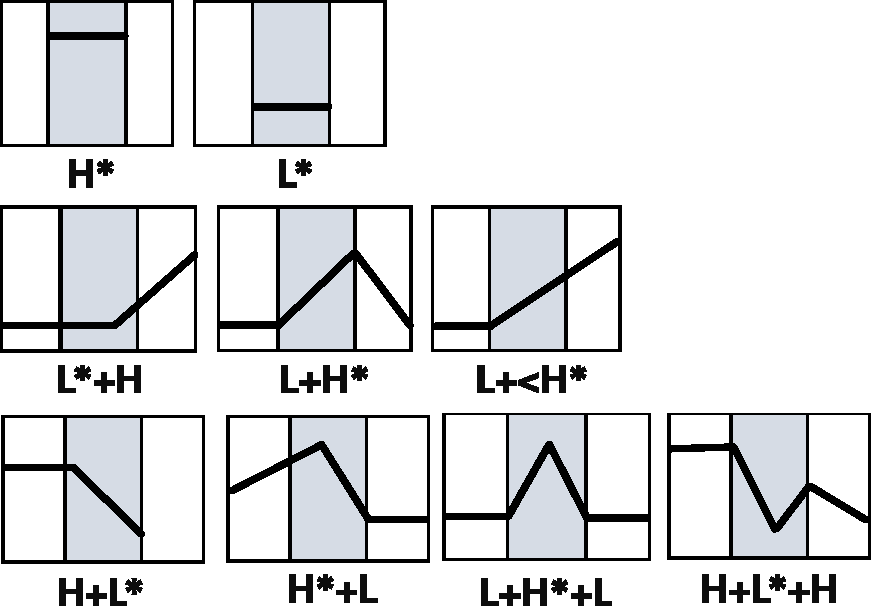
\includegraphics[width=.6\textwidth]{figures/a08HabilAppendix-img002.pdf}


\section{Boundary tones}\label{app:b2}

%%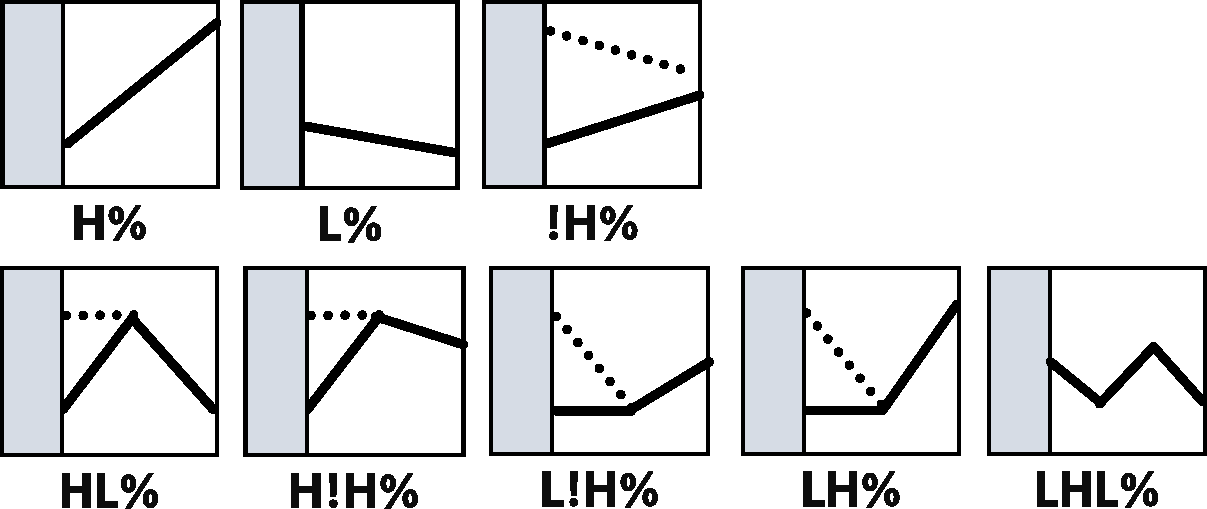
\includegraphics[width=\textwidth]{figures/a08HabilAppendix-img003.emf}
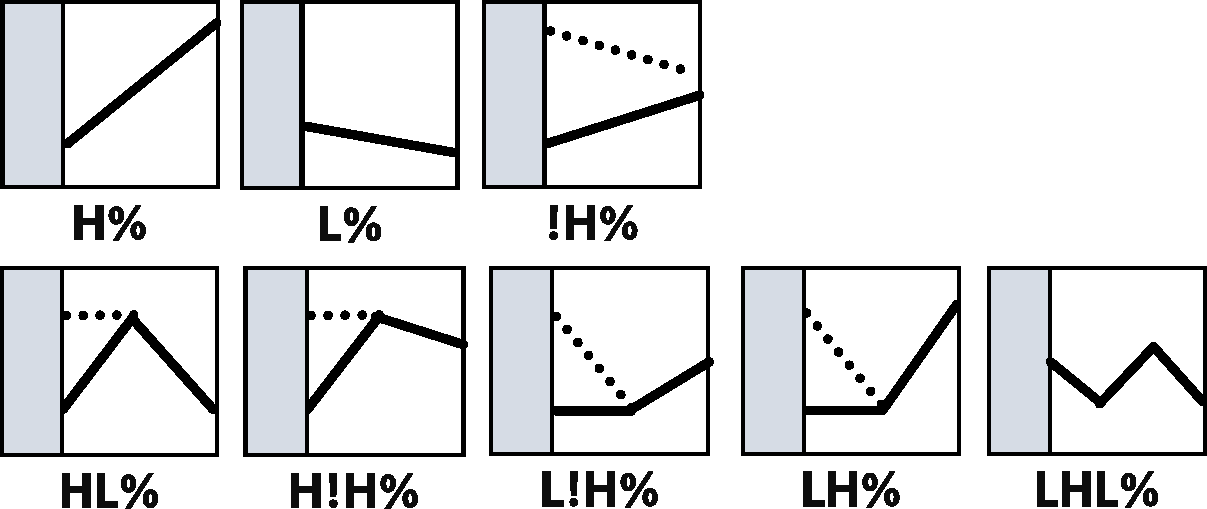
\includegraphics[width=.6\textwidth]{figures/a08HabilAppendix-img003.pdf}
